\chapter{Noise}\label{Noise}
Synthetisch erzeugtes Rauschen \emph{(engl. Noise)} erweist sich als hilfreiches Mittel zur Erzeugung von zufällig erscheinenden Strukturen.
Als wohl bekannteste Implementierung ist hier die Implementierung von Ken Perlin\cite{PERLIN1985} zur Erzeugung einer Marmortextur auf einer Vase zu nennen\footnote{Auch als \emph{Perlin-Noise} bezeichnete Implementierung von Gradient Noise in 3-D}.

Neben umfangreichen Anpassungsmöglichkeiten durch verschiedene Parameter ist die Performance dieses Verfahrens ein entscheidender Grund für die Nutzung. Noise verbraucht extrem wenig Speicher, ist relativ einfach zu berechnen und ist zu jeder Zeit an einer beliebigen Stelle auswertbar, was es auch für Echtzeitanwendungen geeignet macht.\cite{H.Hauser2010}

Dieses Kapitel soll ein grundlegendes Verständnis über Noise-Funktionen bieten. Dazu werden zuerst grundlegende Komponenten, welche jeder Implementierung zugrunde liegen, erläutert. Anschließend werden \emph{Value-}\ref{Value-Noise}, \emph{Gradient-Noise}\ref{Gradient-Noise} sowie \emph{Fractal-Noise}\ref{Fractal-Noise} erklärt, bevor es einen Ausblick auf verschieden Abwandlungen von \emph{Fractal Noise} gibt.

Weitere ausführliche Beschreibung in \cite{BurgerGradientNoise2008} (Gradient-Noise) und in \cite{simplexNoise} zu \emph{Simplex-Noise} welches eine, besonders in höheren Dimensionen, performantere Implementierung von Perlin Noise darstellt.

\section{Grundlagen}
\subsection{Lattice-Function}\label{latticeFunc}
Der erste Schritt zur Erzeugung von Noise ist in der Regel eine sogenannte \emph{Lattice(Gitter)-Funktion}\cite{fractalsAndChaos} der Form \begin{math}l(\vec{k}): {Z}^n \mapsto [-1 - 1]\end{math}\label{latticeFunc}.
Diese dient zur Beschreibung eines Gitters, welches die Form unserer zukünftigen Noise-Funktion bestimmen wird. Die Funktion muss dabei unbedingt deterministisch sein\footnote{Siehe\ref{Fractal-Noise}, sie muss also für jede Koordinate eines Gitterpunktes immer denselben Funktionswert liefern.}. Perlin verwendet bei seiner Implementierung eine Hashfunktion die auf ein, mit zufälligen Werten gefülltes, Array zugreift. Ein Zugriff auf dieses Array mittels simpler Modulo Operation hätte zur Folge, dass sich im Höhenfeld wiederkehrende Strukturen zeigen würden sobald die Funktion über den Rahmen des Arrays hinausgreift.


\subsection{Interpolation und Fade-Function}
Um aufbauend auf der Lattice-Funktion\ref{latticeFunc} eine Funktion $S(\vec{x}): \mathbb{R}^n\mapsto\mathbb{R}, \vec{x}\in \mathbb{Z}^n$\label{S} zu definieren wird zwischen benachbarten Gitterpunkten lokal interpoliert. Dafür wird eine sogenannte Fade-Function\cite{fadeFunction} der Form $f(t): \mathbb{R}\mapsto\mathbb{R}$ mit $t\in[0, 1]$ definiert, welche den Übergang zwischen den Gitterpunkten steuert.

Um überhaupt eine stetige Noise-Funktion zu ermöglichen, muss 
\begin{equation}
f(0) = 0 \land f(1) = 1
\end{equation} gelten.
Damit der Übergang zwischen den Gitterpunkten möglichst glatt und damit natürlich wirkt, sollte jedoch eine Stetigkeit von $C^2$ an den Übergängen und damit die Eigenschaften 
\begin{equation}
	f'(0) = f'(1) = 0 = f''(0) = f''(1)
\end{equation} 
gelten.

Dafür wird im folgenden das Polynom $f(t) = 6t^5-15t^4+10t^3$ benutzt, welches auch in Perlins Referenzimplementierung Verwendung findet\cite{BurgerGradientNoise2008} und alle Eigenschaften erfüllt.
\begin{figure}[!hbtp]%
	\centering
	\begin{tikzpicture}
		\begin{axis}
			[ 
				xlabel=$t$,
				ylabel={$f(t) = 6t^5-15t^4+10t^3$},
				ymin=0,
				ymax=1,
				xmin=0,
				xmax=1,
				restrict x to domain=0:1
			] 
			
			\addplot[no markers, blue, smooth, domain = 0:1] {x * x * x * (x * (x * 6 - 15) + 10)}; 
		\end{axis}
	\end{tikzpicture}
	\caption{Fade-Function}
\end{figure}


\section{Value-Noise}\label{Value-Noise}
Value-Noise ist die wohl naivste Implementierung einer Noise-Funktion. Bei ihr werden die Gitterpunktwerte, welche durch die \emph{Lattice-Funktion}\ref{latticeFunc} erzeugt wurden, als Höhenwerte interpretiert.

Die mit $f(t)$ gebildete, interpolierende Funktion $vnoise(\vec{x}) = noise(\vec{x})$ definiert nun die Value-Noise-Funktion.

Untenstehend ist eine Implementierung in C\# für eine Zweidimensionale Rauschfunktion zu sehen.
Noise lässt sich problemlos in mehrere Dimensionen skalieren. Einzig die Interpolation der Werte muss hier angepasst werden. In der Implementierung ist zu sehen, wie die Gitterpunktwerte - ähnlich einer \emph{billinearen Interpolation} - mit der \emph{Fade-Function} interpoliert werden.

\lstinputlisting[language=csh, title=Value-Noise Implementierung C\#]{data/valueNoise.cs}\label{valueNoise.cs}

\section{Gradient-Noise}\label{Gradient-Noise}
Der vorher erwähnte Value-Noise kann, je nach Parameterwahl, noch ein unruhiges Rauschen erzeugen. Um die Übergänge zwischen den Gitterpunktwerten noch sanfter und damit natürlicher aussehen zu lassen wurde der Gradient-Noise erfunden.
Hier werden die Gitterpunktwerte nicht als Höhenwerte, Gradienten an den Nullstellen der Noise-Funktion gesehen.
Es ergibt sich also:
\begin{equation}
noise(\vec{k}) = 0 \land 
noise'(\vec{k}) = gnoise(\vec{k}),  k \in \mathbb{Z}^n  .
\end{equation}

In der untenstehenden 2D C\# Implementierung ist zu sehen, wie zuerst ein Höhenwert für den aktuellen Punkt  $\vec{x}$ über das Skalarprodukt\footnote{engl. Dot-Product} zwischen dem Gradienten und der relativen Position $\begin{pmatrix}tx\\ty\end{pmatrix}  tx, ty\in [0-1]$ und anschließend über die bekannte Interpolation berechnet wird.

\lstinputlisting[language=csh, title=Gradient-Noise Implementierung C\#]{data/gradientNoise.cs}
 

\section{Fractal-Noise}\label{Fractal-Noise}

Die bisher behandelten Noise-Funktionen erzeugen zwar natürlich erscheinende Zufallswerte, wenn man diese jedoch auf eine Heightmap überträgt wird deutlich, dass es ihr an Details fehlt um realistisch zu wirken.

Um den Detailgrad der Noise-Funktion beliebig zu erhöhen, wird sie mit einer gestauchten, in der Amplitude verringerten, Version ihrer selbst addiert. 
Dieses Verfahren lässt sich beliebig oft anwenden, was einen hohen Detailgrad erlaubt.
Die verschiedenen Frequenzen die dadurch entstehen werden wegen der Halbierung bzw. Verdopplung bei Perlins Implementierung\footnote{$L=2$} auch als \emph{Oktaven} bezeichnet.

In \cite{Saupe} wird daher folgende Formel definiert:
\begin{equation} \label{eq.fractalnoise}
	fractal(\vec{x}) = \sum_{k=k_0}^{k_1}\frac{1}{r^{kH}}gnoise(r^k\vec{x}).
\end{equation}

Wobei $H=2-D$ der Hurst-Exponent ist\cite{tuMuenchen} und %TODO S. 438 oder so nachgucken wegen H
$D=-\frac{log(\frac{1}{k1})}{log(r)}$\cite{fraktDim} die fraktale Dimension.

In der Formel beschreibt $r$ die sogenannte Lacunarity. Mit ihr lässt sich steuern, wie stark die Amplitude bei jeder Oktave abnimmt bzw. sich die Frequenz erhöht.
Durch die Anpassung dieser Parameter lässt sich das Verhalten der Noise-Funktion gezielt steuern. Eine Implementierung in C\# findet sich unten.

\begin{figure}
	\centering
	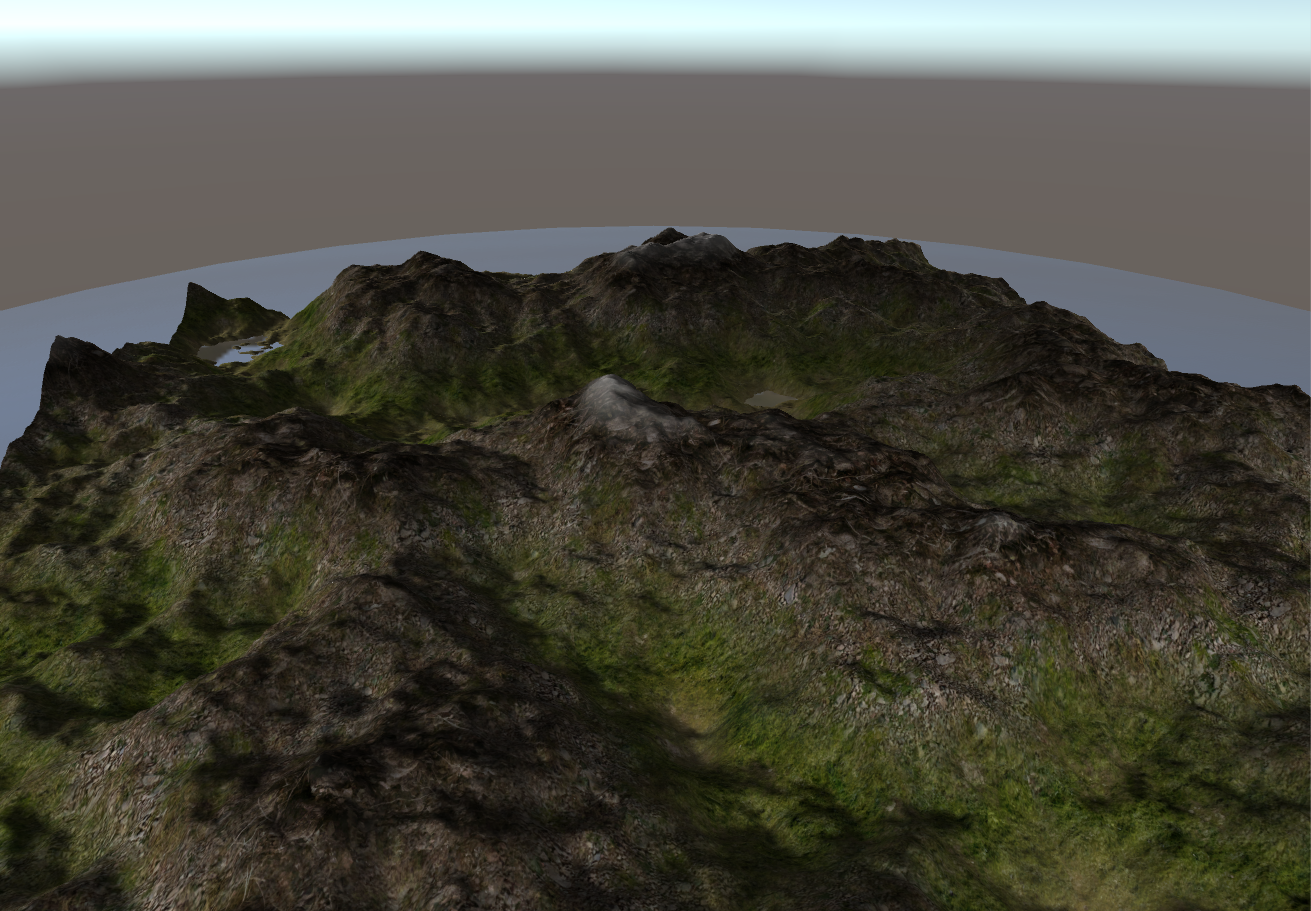
\includegraphics[width=\textwidth]{images/perlin_rendered.png}
	\caption{Texturierte Landschaft im Beispielprogramm die aus fraktalem Perlin-Noise entstanden ist.}\label{img.perlinRendered}
\end{figure}

\lstinputlisting[language=csh, title=Simple Fractal-Noise Implementierung C\#]{data/fractalNoise.cs}

\section{Noise-Variationen}\label{NoiseVariationen} %TODO Screenshots der Noise Variationen
Die in \ref{eq.fractalnoise} beschriebene Funktion lässt sich beliebig erweitern und anpassen um bestimmte Effekte zu erzielen. Im folgenden sollen daher einige bekannte und für Landschaften passende Erweiterungen erläutert werden. Diese Auflistung ist nur als eine Auswahl zu verstehen. Es gibt noch zahlreiche weitere Implementierungen wie z.B. Convolution oder auch sparse Convolution-Noise\cite{texturingAndModeling}.

\subsection{Ridged-Noise}
In der Natur lassen sich in einigen Gebirgen sehr steile und gezahnte Kämme feststellen. Aufgrund der kontinuierlichen Natur einer Noise-Funktion sind die Kämme jedoch eher abgerundet. 
Um diesen Effekt aufzuheben wird der Betrag der Noise-Funktion von 1 abgezogen. 

\begin{equation} \label{eq.ridgedNoise}
ridged(\vec{x}) = \sum_{k=k_0}^{k_1}\frac{1}{r^{kH}}(1-\left|gnoise(r^k\vec{x})\right|).
\end{equation}

Anschaulich modelliert die Funktion nun Material aus einem Quader heraus anstatt die Landschaft auf eine Ebene rauf zu modellieren. Durch den Betrag verliert die Funktion außerdem ihre Stetigkeit in der ersten Ableitung, was zu einem abrupten Richtungswechseln der Höhenfunktion führt. An diesen Punkten entstehen nun, wie in \autoref{img.ridgedRendered}zu sehen, die erwünschten scharfen Kämme.

\begin{figure}
	\centering
	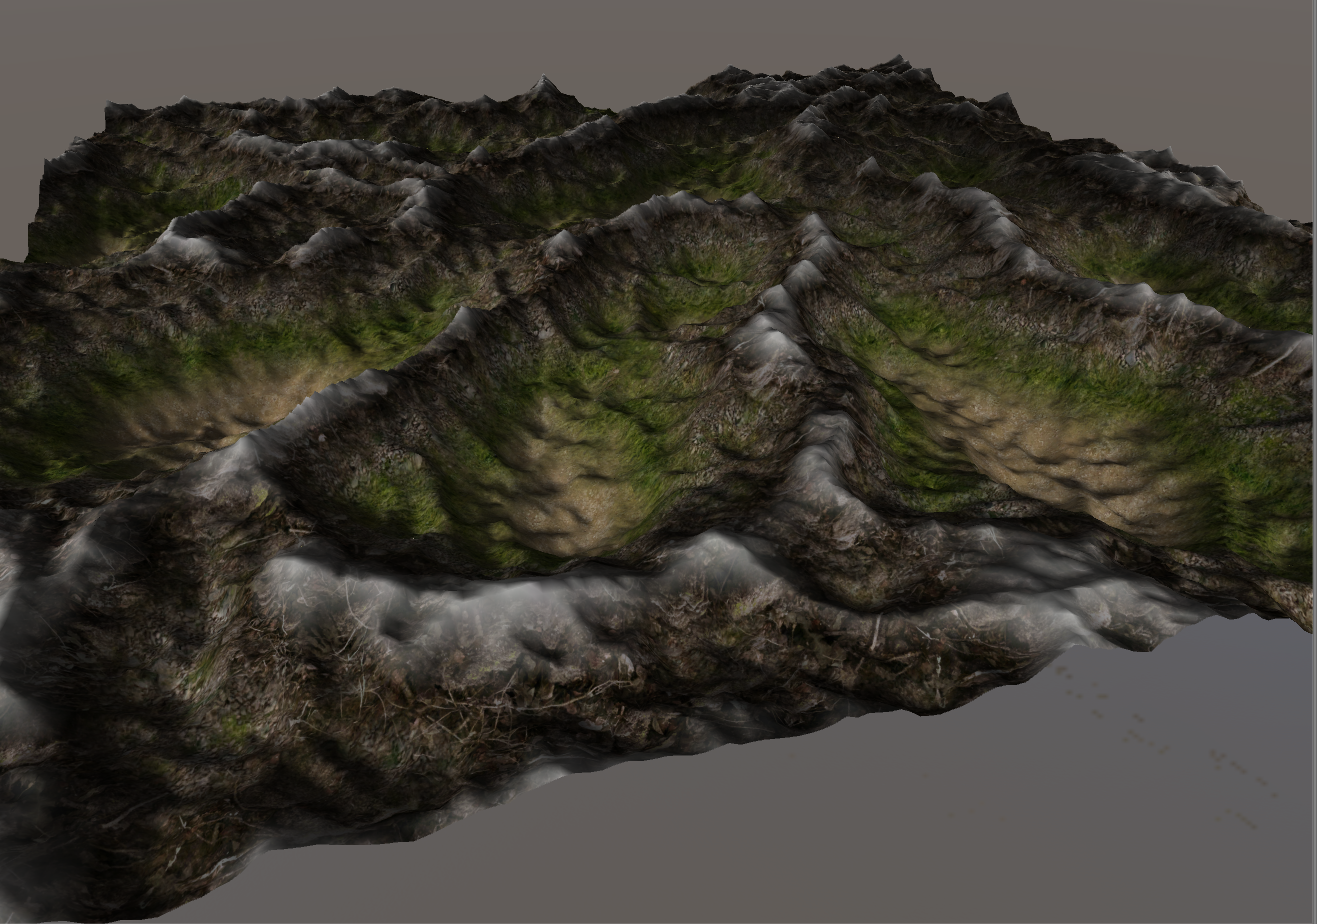
\includegraphics[width=\textwidth]{images/ridged_rendered.png}
	\caption{Texturierte Landschaft im Beispielprogramm die aus Ridged Noise entstanden ist}\label{img.ridgedRendered}
\end{figure}

\lstinputlisting[language=csh, title=Ridged-Noise Implementierung HLSL]{data/RidgedNoiseHLSL.hlsl}

\subsection{Multifraktal/heterogenes Terrain}
Wie auch in \ref{unisotrop} erwähnt kommen hohe Frequenzen momentan sowohl in den Tälern als auch auf den Bergen unserer Landschaft vor. Um diese homogenität zu verhindern wurde eine Noise Funktion entwickelt die durch Multiplikation der Oktaven zu einem Multifraktal führt\footnote{\cite{texturingAndModeling} p.440}. 

\begin{equation} \label{eq.fractalnoise}
multi(\vec{x}) = \prod_{k=k_0}^{k_1}\frac{1}{r^{kH}}(gnoise(r^k\vec{x})+o).
\end{equation}

Es ist hierbei anzumerken, dass das Intervall des Ergebnisses dieser Rauschfunktion stark variiert. Um ein Ergebnis in einem konstanten Intervall zu verarbeiten muss im Nachhinein der höchste bzw. tiefste Punkt gesucht werden und entsprechend skaliert werden. Dadurch geht der Vorteil der parallelen Berechnung zur Echtzeit verloren. Eine andere Möglichkeit ist den Parameter $o$ entsprechend anzupassen um das Ergebnis in eine bestimmte Richtung zu beeinflussen. 
In \autoref{img.multiRendered} ist zu sehen, wie die tiefer gelegenen Gebiete deutlich weniger Anteile von hohen Frequenzen aufweisen und dadurch natürlicher wirken.

\begin{figure}
	\centering
	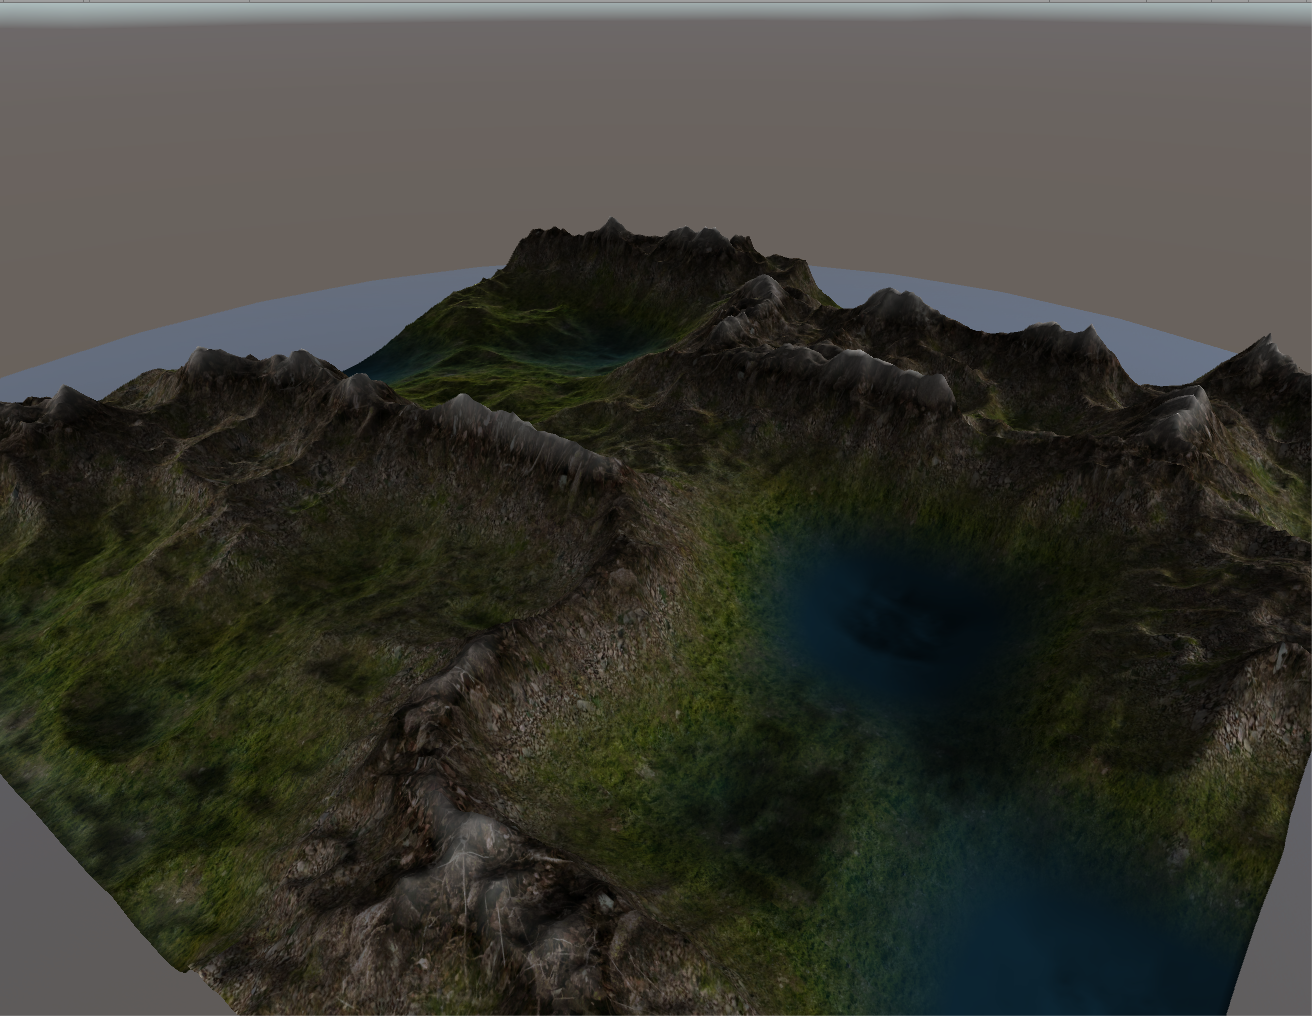
\includegraphics[width=\textwidth]{images/ridgedmulti_rendered.png}
	\caption{Texturierte Landschaft im Beispielprogramm die aus Ridged-Multifractal-Noise mit $o=0.2$ entstanden ist.}\label{img.multiRendered}
\end{figure}

\lstinputlisting[language=csh, title=Ridged-Multifractal Noise Implementierung HLSL]{data/RidgedMultiNoiseHLSL.hlsl}

\subsection{Hybrid-Multifractal}
Um das Problem des schwer zu bestimmenden Intervalls einer Multifraktalen Rauschfunktion zu umgehen und trotzdem ein heterogenes Terrain Ergebnis zu erzielen lassen sich die normale und die Multifraktale Rauschfunktion auch kombinieren. 
Die Heterogenität lässt sich dadurch erreichen, dass jede Oktave vor der Addition mit einem Gewicht multipliziert wird, welches das Produkt der vorherigen Oktaven ist. Dabei wird ein Faktor $w$ definiert, welcher das zu schnelle abfallen des Gewichtwertes bremst.

In \autoref{img.hybridmultiRendered} ist zu sehen, dass die hohen Frequenzen wie beim Multifraktalem Rauschen kaum noch Einfluss in den Tälern haben.

\begin{figure}
	\centering
	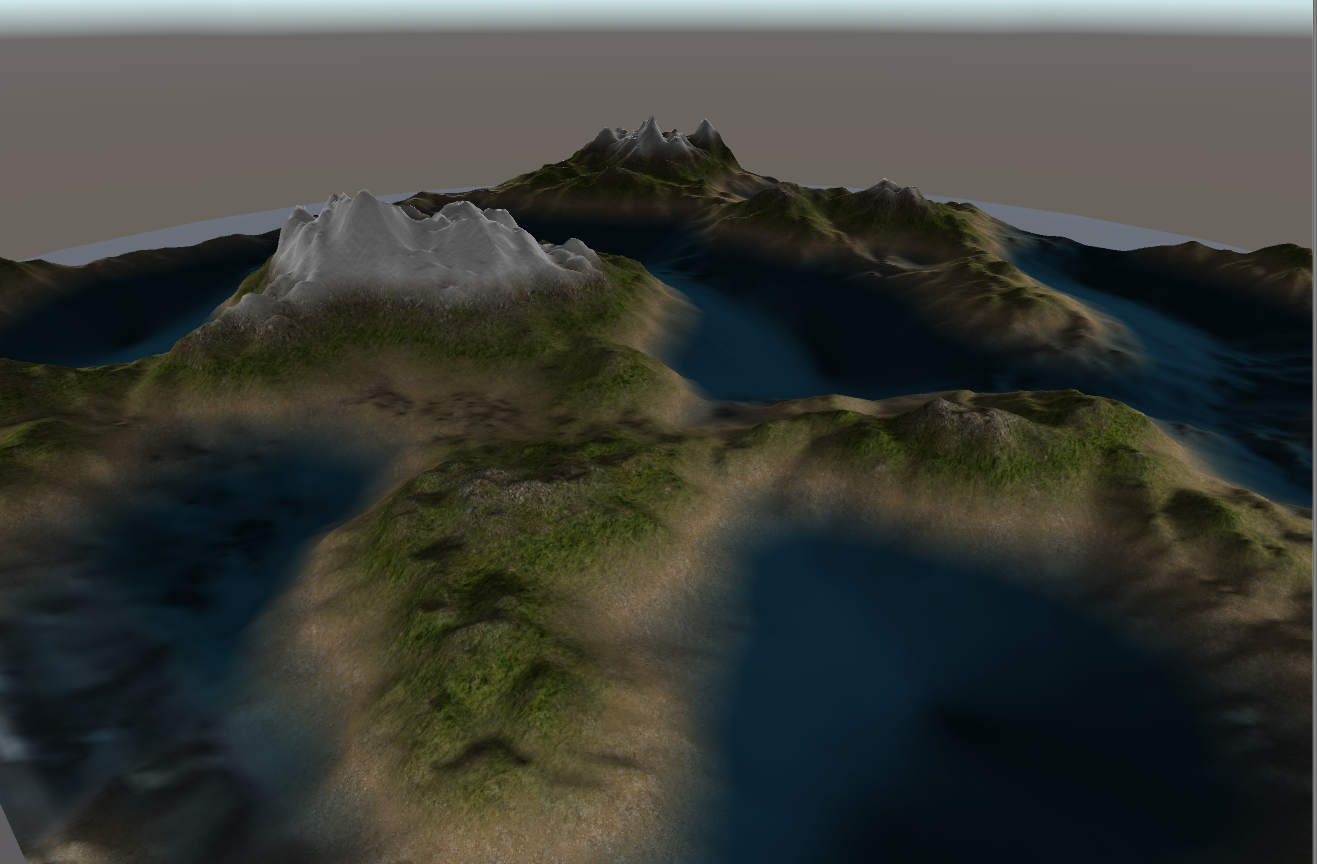
\includegraphics[width=\textwidth]{images/hybridmulti_rendered.png}
	\caption{Texturierte Landschaft im Beispielprogramm die aus Hybrid-Multifractal-Noise mit $o=0.5$ entstanden ist.}\label{img.hybridmultiRendered}
\end{figure}

\lstinputlisting[language=csh, title=Hybrid-Multifractal Noise Implementierung HLSL]{data/HMFNoise.hlsl}


\subsection{Domain/Range Mapping}
%Dummy text
Um das Problem des schwer zu bestimmenden Intervalls einer Multifraktalen Rauschfunktion zu umgehen und trotzdem ein heterogenes Terrain Ergebnis zu erzielen lassen sich die normale und die Multifraktale Rauschfunktion auch kombinieren. 
Die Heterogenität lässt sich dadurch erreichen, dass jede Oktave vor der Addition mit einem Gewicht multipliziert wird, welches das Produkt der vorherigen Oktaven ist. Dabei wird ein Faktor $w$ definiert, welcher das zu schnelle abfallen des Gewichtwertes bremst.

In \autoref{img.hybridmultiRendered} sieht man, dass die hohen Frequenzen wie beim Multifraktalem Rauschen  kaum noch Einfluss in den Tälern haben.
%TODO Fertig machen

\begin{figure}
	\centering
	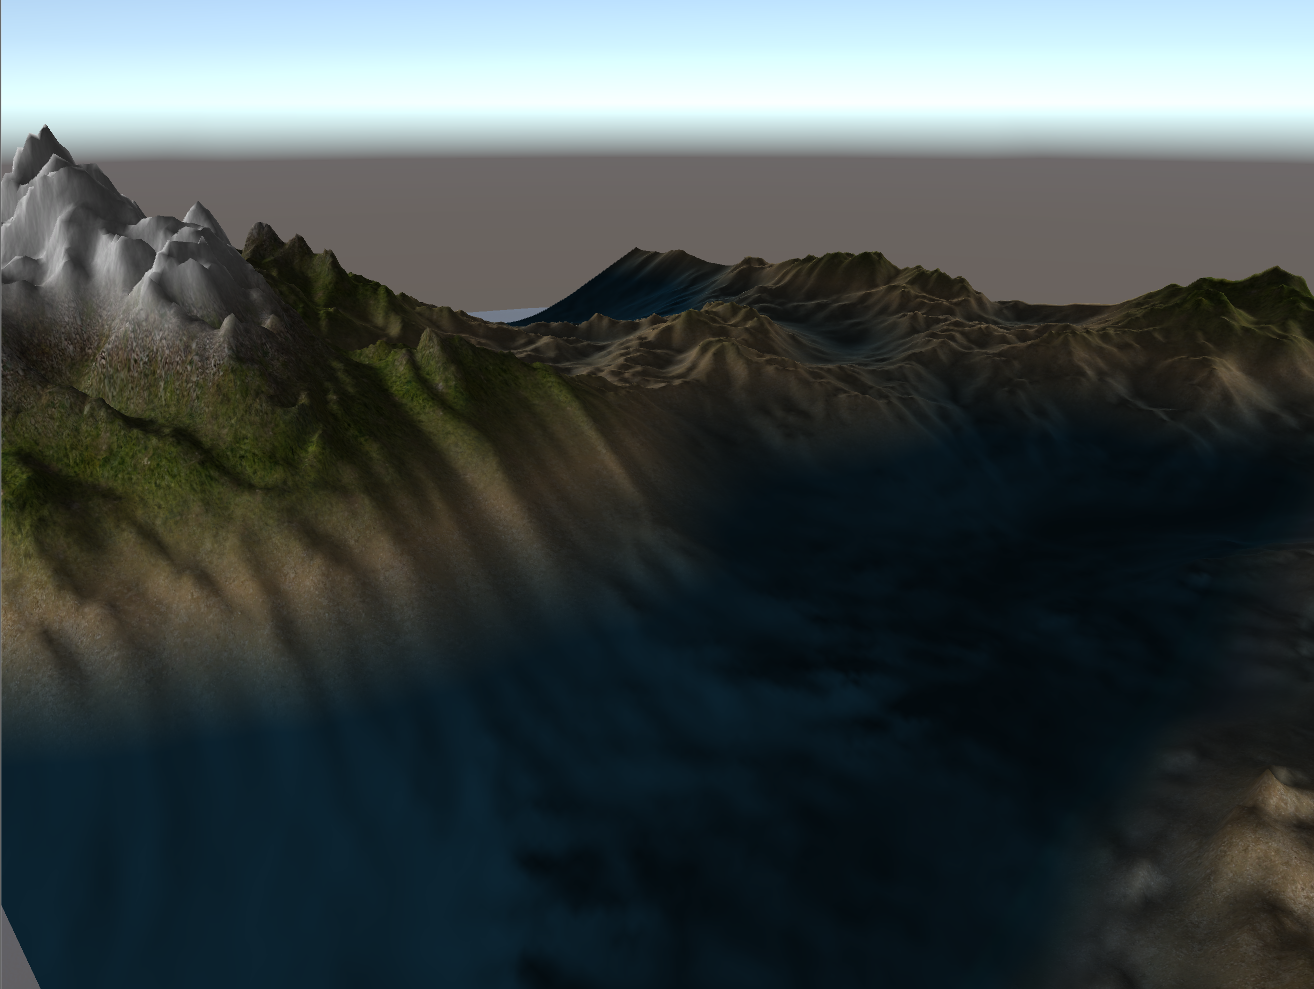
\includegraphics[width=\textwidth]{images/domainwarped_rendered.png}
	\caption{Texturierte Landschaft im Beispielprogramm die aus Domain Mapped Multifractal-Noise mit $o=0.48$ und $\alpha=20$ entstanden ist.}\label{img.multiRendered}
\end{figure}


%TODO Auflistung und Bilder der Ergebnisse






